    \newcommand{\width}{0.2}
    
\tikzset{sigmoid/.style={path picture= {
    \begin{scope}[x=1pt,y=10pt]
      \draw plot[domain=-7:7] (\x,{1/(1 + exp(-\x))-0.5});
    \end{scope}
    }
  }
}

\tikzset{relu/.style={path picture= {
    \begin{scope}[x=7pt,y=6pt]
      \draw plot[domain=-1:0] (\x,0);
      \draw plot[domain=0:1] (\x,\x);
    \end{scope}
    }
  }
}

\tikzstyle{input}=[draw,fill=red!50,circle,minimum size=20pt,inner sep=0pt]
\tikzstyle{hidden}=[draw,fill=white,circle,minimum size=20pt,inner sep=0pt]
\tikzstyle{output}=[draw,fill=white,circle,minimum size=20pt,inner sep=0pt]
\tikzstyle{bias}=[draw,dashed,fill=gray!50,circle,minimum size=20pt,inner sep=0pt]
\tikzstyle{layer}=[fill=gray!70]

\tikzstyle{stateTransition}=[->, thick]

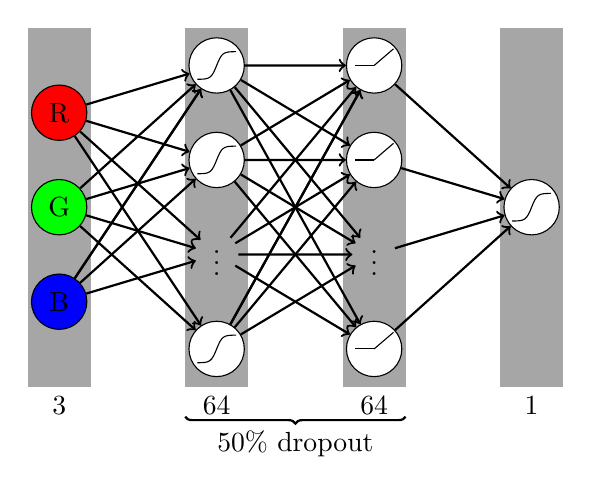
\begin{tikzpicture}[scale=2,yscale=0.6]
    \fill[layer] (  -\width,-1.9) rectangle (  \width,1.9);
    \fill[layer] (1+-\width,-1.9) rectangle (1+\width,1.9);
    \fill[layer] (2+-\width,-1.9) rectangle (2+\width,1.9);
    \fill[layer] (3+-\width,-1.9) rectangle (3+\width,1.9);
    \node (l1label) at  (0, -2.1) {3};
    \node (l2label) at  (1, -2.1) {64};
    \node (l3label) at  (2, -2.1) {64};
    \node (l4label) at  (3, -2.1) {1};
    \node (r)[input,fill=red]   at (0, 1) {R};
    \node (g)[input,fill=green] at (0, 0) {G};
    \node (b)[input,fill=blue]  at (0,-1) {B};

    \node (h11)[hidden, sigmoid] at (1, 1.5) {};
    \node (h12)[hidden, sigmoid] at (1, 0.5) {};
    \node[circle, inner sep=0] (h13) at (1,-0.5) {\vdots};
    \node (h14)[hidden, sigmoid] at (1,-1.5) {};
    \node (h21)[hidden, relu] at (2, 1.5) {};
    \node (h22)[hidden, relu] at (2, 0.5) {};
    \node[circle, inner sep=0] (h23) at (2,-0.5) {\vdots};
    \node (h24)[hidden, relu] at (2,-1.5) {};

    \node (o1)[output, sigmoid] at (3,0) {};

    \draw[stateTransition] (r) -- (h11) node [midway,above=-0.06cm] {};
    \draw[stateTransition] (r) -- (h12) node [midway,above=-0.06cm] {};
    \draw[stateTransition] (r) -- (h13) node [midway,above=-0.06cm] {};
    \draw[stateTransition] (r) -- (h14) node [midway,above=-0.06cm] {};
    \draw[stateTransition] (g) -- (h11) node [midway,above=-0.06cm] {};
    \draw[stateTransition] (g) -- (h12) node [midway,above=-0.06cm] {};
    \draw[stateTransition] (g) -- (h13) node [midway,above=-0.06cm] {};
    \draw[stateTransition] (g) -- (h14) node [midway,above=-0.06cm] {};
    \draw[stateTransition] (b) -- (h11) node [midway,above=-0.06cm] {};
    \draw[stateTransition] (b) -- (h12) node [midway,above=-0.06cm] {};
    \draw[stateTransition] (b) -- (h13) node [midway,above=-0.06cm] {};
    \draw[stateTransition] (b) -- (h11) node [midway,above=-0.06cm] {};

    \draw[stateTransition] (h11) -- (h21) node [midway,above=-0.06cm] {};
    \draw[stateTransition] (h11) -- (h22) node [midway,above=-0.06cm] {};
    \draw[stateTransition] (h11) -- (h23) node [midway,above=-0.06cm] {};
    \draw[stateTransition] (h11) -- (h24) node [midway,above=-0.06cm] {};
    \draw[stateTransition] (h12) -- (h21) node [midway,above=-0.06cm] {};
    \draw[stateTransition] (h12) -- (h22) node [midway,above=-0.06cm] {};
    \draw[stateTransition] (h12) -- (h23) node [midway,above=-0.06cm] {};
    \draw[stateTransition] (h12) -- (h24) node [midway,above=-0.06cm] {};
    \draw[stateTransition] (h13) -- (h21) node [midway,above=-0.06cm] {};
    \draw[stateTransition] (h13) -- (h22) node [midway,above=-0.06cm] {};
    \draw[stateTransition] (h13) -- (h23) node [midway,above=-0.06cm] {};
    \draw[stateTransition] (h13) -- (h24) node [midway,above=-0.06cm] {};
    \draw[stateTransition] (h14) -- (h21) node [midway,above=-0.06cm] {};
    \draw[stateTransition] (h14) -- (h22) node [midway,above=-0.06cm] {};
    \draw[stateTransition] (h14) -- (h23) node [midway,above=-0.06cm] {};
    \draw[stateTransition] (h14) -- (h21) node [midway,above=-0.06cm] {};

    \draw[stateTransition] (h21) -- (o1) node [midway,above=-0.06cm] {};
    \draw[stateTransition] (h22) -- (o1) node [midway,above=-0.10cm] {};
    \draw[stateTransition] (h23) -- (o1) node [midway,above=-0.06cm] {};
    \draw[stateTransition] (h24) -- (o1) node [midway,above=-0.06cm] {};

    \draw [
    thick,
    decoration={
        brace,
        mirror,
        raise=0.5cm
    },
    decorate
] (1+-\width, -1.8) -- (2+\width, -1.8)
node [pos=0.5,anchor=north,yshift=-0.55cm] {50\% dropout};
\end{tikzpicture}